% !TEX program = xelatex
%% Requires compilation with XeLaTeX or LuaLaTeX
\documentclass[10pt,xcolor={table,dvipsnames},t]{beamer}
\usepackage{biblatex}
\usepackage{caption}
\setbeamertemplate{caption}[numbered]
\addbibresource{reference.bib}
\usepackage{hyperref}
\hypersetup{ 
pdfpagemode=FullScreen,  
colorlinks=true,linkcolor=blue}
\usepackage{enumerate}

\usepackage{listings}
\usepackage{xcolor}

\definecolor{codegreen}{rgb}{0,0.6,0}
\definecolor{codegray}{rgb}{0.5,0.5,0.5}
\definecolor{codepurple}{rgb}{0.58,0,0.82}
\definecolor{backcolour}{rgb}{0.95,0.95,0.92}

\lstdefinestyle{mystyle}{
    backgroundcolor=\color{backcolour},   
    commentstyle=\color{codegreen},
    keywordstyle=\color{magenta},
    numberstyle=\tiny\color{codegray},
    stringstyle=\color{codepurple},
    basicstyle=\ttfamily\footnotesize,
    breakatwhitespace=false,         
    breaklines=true,                 
    captionpos=b,                    
    keepspaces=true,                 
    numbers=left,                    
    numbersep=5pt,                  
    showspaces=false,                
    showstringspaces=false,
    showtabs=false,                  
    tabsize=2
}

\lstset{style=mystyle}

\usetheme{UCBerkeley}

\title[Your Short Title]{STMC coding team training}
\subtitle{Lesson 1: Hello World}
\author{Tsai Yun Chen}
%\institute{}
\date{\today}

\begin{document}

\begin{frame}
  \titlepage
\end{frame}

% Uncomment these lines for an automatically generated outline.
%\begin{frame}{Outline}
%  \tableofcontents
%\end{frame}

\section{Class Goal}

\begin{frame}{What we are going to do today?}

\begin{enumerate}
  \item Setup Environment for coding
  \item Run your first program \texttt{helloworld.ipynb}
  \item Understand different parts of \texttt{helloworld.ipynb}
\end{enumerate}
%\begin{block}{Examples}
%Some examples of commonly used commands and features are included, to help you get started.
%\end{block}

\end{frame}

\section{Installing python}

\begin{frame}{Tools we are going to use}
  \begin{itemize}
    \item As mentioned we need a compiler to translate our program to machine code
    \item Unfortunately we do not have compiler installed in our computer yet
    \item To solve this, we are going to use a online tool named \texttt{Google Colab}
  \end{itemize}
\end{frame}

\begin{frame}{What is Google Colab}
  \begin{itemize}
    \item Google Colab is a online notebook provided by Google
    \item allows user to write and run python code online
    \item It has several benefit over traditional local compiler:
    \begin{enumerate}
      \item code everywhere
      \item free GPU usage
      \item can share your code to others and work together (like google doc)
    \end{enumerate}
  \end{itemize}
\end{frame}

\begin{frame}[fragile]{What you need to do}
  \begin{columns}
    \column{0.8\textwidth}
    \begin{enumerate}[Step 1:]
      \item prepare a Google account
      \item Login your Google account and go to your Google drive
      \item Open a new folder to hold the files that you will use in this course
    \end{enumerate}
  \end{columns}
\end{frame}


\section{Running your first program}
\begin{frame}{Running your first program (I)}
  \begin{columns}
    \column{0.8\textwidth}
    \begin{enumerate}[Step 1:]
      \item Download \texttt{HelloWorld.ipynb} from course webpage.
      \item Upload the file you just downloaded to the Google drive folder
      \item double click to open the file when the upload is finished
    \end{enumerate}
  \end{columns}
\end{frame}

\begin{frame}[fragile]{Running your first program (II)}
  Now you should see the page below, click the start button beside the code:
\vspace{1mm}
You should see the following results:
\begin{lstlisting}
  Hello world!
\end{lstlisting}
\begin{figure}
  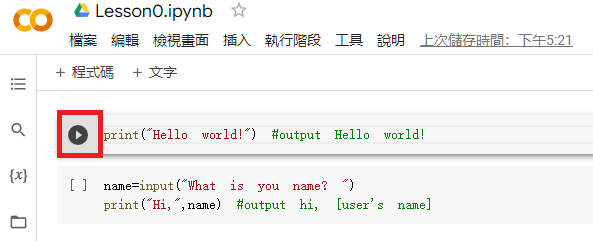
\includegraphics[width=0.8\textwidth]{img/driveAddCollab.png}
\end{figure}
\end{frame}


\section{Understanding helloworld.py}
% \begin{frame}[fragile]{Understand helloworld.py}
%   Congrats, you just compile your first program. Now, let's open \texttt{helloworld.py} and see what's under the hood:
%   \begin{lstlisting}[language=python]
%     print("Hello world!") #output Hello world!
%     #name=input("What is you name?\n") #ask for your name
%     #print("Hi,",name) #output hi, [user's name] #output hi, [user's name]
% \end{lstlisting}
% \end{frame}

\begin{frame}[fragile]{Experiments}
   Congrats, you just compile your first program. Now, let's explore the function of different parts of the program by doing some experiments:
  \begin{enumerate}
    \item Change "Hello World" to "Bye bye world" and rerun, what do you observe?
    \item Similar to the first line, add more \texttt{print} to see if you can print multiple lines
    \item Change the text behind \# in line 1 and recompile, does it change anything about the code? Now try to add \# before \texttt{print}, what happens?
  \end{enumerate}
\end{frame}

\begin{frame}[fragile]{Explaining helloworld.py: print}
  \begin{itemize}
    \item \texttt{print} is a function used for printing things
    \item In \texttt{helloworld.py}, \texttt{print} is used to print our hello message "Hello world"
    \item You can also do something like this:
\begin{lstlisting}[language=python]
  print("Text 1", "Text 2", "Text 3")
\end{lstlisting}
    These text will be separated by spaces (Try it!)
    \item You can read more about \texttt{print} from the \href{https://docs.python.org/3/library/functions.html#print}{documentation}
  \end{itemize}
\end{frame}

\begin{frame}{Explaining helloworld.py : Comments}
  \begin{itemize}
    \item Those lines after \texttt{\#} are called \textbf{comments}
    \item They are ignored by compiler and will not affect how the code run
    \item Their are notes left by programmers to help himself/herself/others to understand the code 
    \item \textbf{For more complicated program, comments are necessary}. Otherwise, code will be very difficult to comprehend and debug
  \end{itemize}
\end{frame}

\begin{frame}[fragile]{Second step}
  \begin{itemize}
    \item Now the computer knows how to talk with you, but we can't talk to the computer !?
    \item Next step we are going to communicate with it, slightly click any blank space of the second block
    \item then you should see the start button appear at the left side similar to what you just did, now click it
    \item the computer will probably ask you a question, answer it by typing, click enter after your input and see what it answer.
  \end{itemize}
\end{frame}

\begin{frame}[fragile]{Explaining helloworld.py : Input}
  \begin{itemize}
    \item As you can probably see, \texttt{input} ask you a question which you can answer 
    \item You answer by typing some input and press enter to submit
    \item Furthermore, the text inside \texttt{input} is displayed when it prompts for answer
    \item So in our program you see the following line is acutally asking your name and waiting for you input:
    \begin{lstlisting}[language=python]
      input("What is your name? ")
\end{lstlisting}
    \item But here is a problem: How can we save and manipulate these input?
  \end{itemize}
\end{frame}
\begin{frame}{Variables - Your handy storage box}
  \begin{itemize}
    \item Imagine that if you never remember things, then how can you answer questions?
    \item To store data, a computer uses something called a \textbf{variable}
    \item A variable is a ”storage box” with a name
    \item It stores data temporarily so that the value inside can be retrieved for further processing
  \end{itemize}
  \begin{figure}
    \centering 
    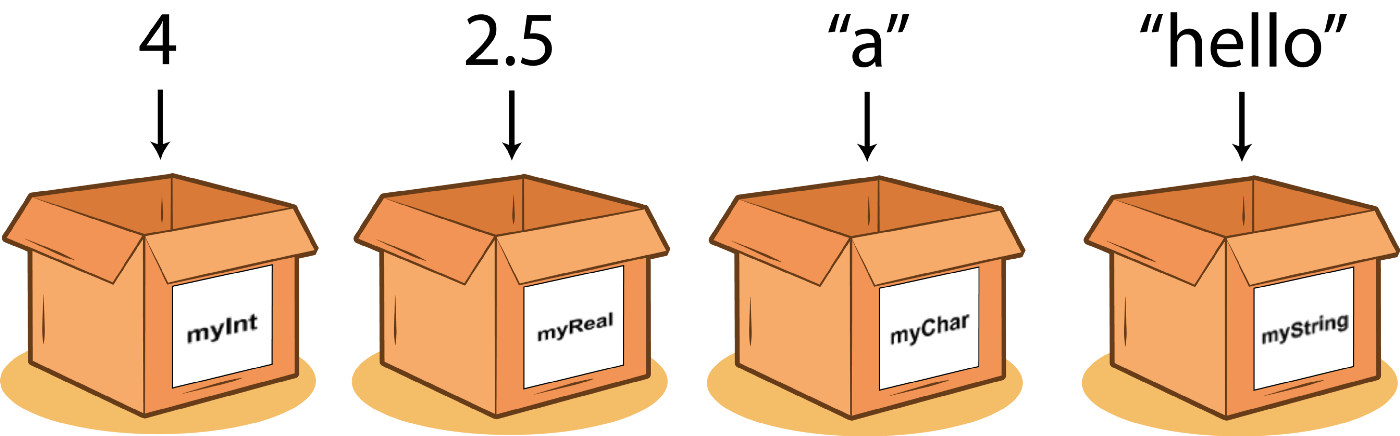
\includegraphics[width=0.6\textwidth]{img/variable.png}
    \caption*{Source: \href{https://stevenpcurtis.medium.com/what-is-a-variable-3447ac1331b9}{https://stevenpcurtis.medium.com/what-is-a-variable-3447ac1331b9}}
  \end{figure}
\end{frame}
\begin{frame}[fragile]{Explaining helloworld.py : Input}
  \begin{itemize}
    \item So back to our example, we see that the full line of our program is actually
    \begin{lstlisting}[language=python]
      name=input("What is your name? ")\end{lstlisting}
    \item now we know that name is a variable that stores your input, which is your name.
    \item Further we see the line follows,
    \begin{lstlisting}[language=python]
      print("Hi,",name)\end{lstlisting}
    \item here we are trying to response to what user input
    \item so refering to our experiment before we can expect the response is what we expect in the comment: \texttt{Hi, [your\_name]}
  \end{itemize}
\end{frame}

\begin{frame}[fragile]{More experiments}
  Let's try out something more:
  \begin{itemize}
    \item Change the variable \texttt{name} to sth else, say your favorite character or song or etc, does the code still works?
    \item try to input something else when answering the question, like entering number, what you expect to get?
    \item can youy modify the code to ask more question? thens print out all the information you gather in one line.
  \end{itemize}
\end{frame}
\end{document}
